\section{Time Estimation}
\label{sec:timeEst}
This section elaborates on the calculation of the time estimation. This time estimation is calculated per motor from which the highest time estimation is used to synchronize all the motors.

To estimate the time needed to reach a target, two situations have to be considered, with $v_0$ the initial velocity, $v_{max}$ the maximum allowable velocity of that motor and $v_{target}$ the final velocity of that motor:
\begin{enumerate}
    \item $v_{max}$ is reached;
    \item $v_{max}$ is not reached.
\end{enumerate}

\noindent Whether or not $v_{max}$ can be reached can be checked with $t_{crit,0}$/$t_{crit,target}$ and $s_{crit}$, where $t_{crit,x}$ is the time required to reach $v_{max}$ from $v_x$ and $s_{crit}$ is the distance travelled when reaching $v_{max}$ from $v_0$ and immediately decelerating to $v_{target}$ (i.e., a bang-bang-trajectory). This type of trajectory is shown in \cref{fig: MSC_crit}, where the area under $v(t)$ is equal to $s_{crit}$. 

\begin{figure}[!hbt]
    \centering
    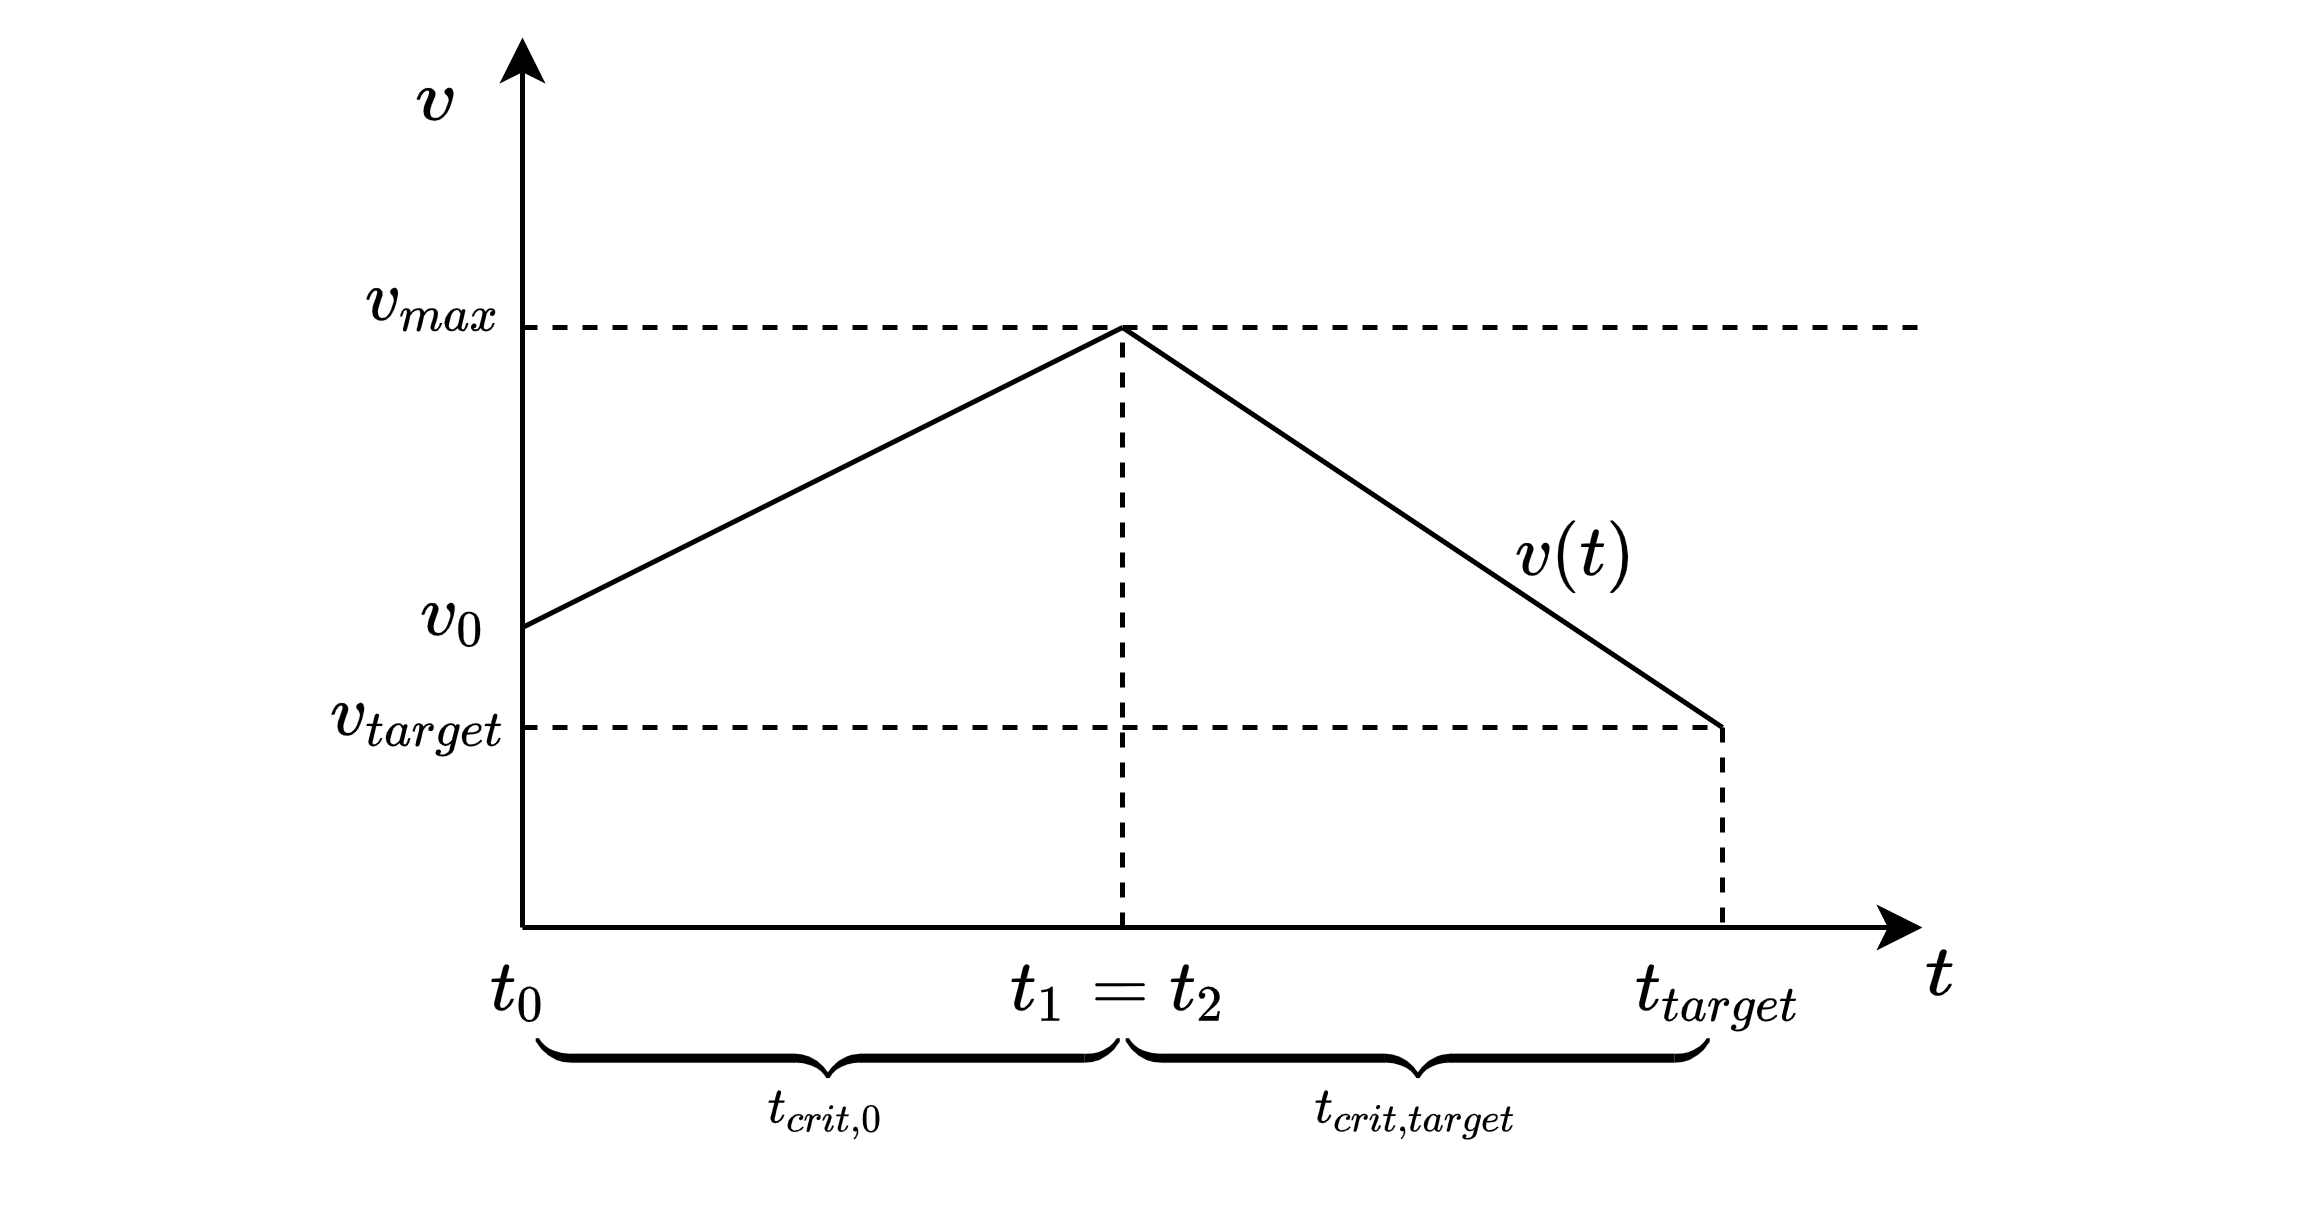
\includegraphics[width=0.7\textwidth]{figures/MotorSpeedCalculations/MSC_crit_trajectory.png}
    \caption{Critical trajectory when reaching maximum speed.}
    \label{fig: MSC_crit}
\end{figure}

\noindent Expressed in the given terms, $t_{crit,0}$/$t_{crit,target}$ can be found as shown in \cref{eq: tCrit}, and $s_{crit}$ can be found as shown in \cref{eq: sCrit}. 
\begin{align}
    t_{crit,x} &= \frac{\Delta v}{a_{max}} = \frac{v_{max}-v_x}{a_{max}} \Rightarrow t_{crit,0} = \frac{v_{max} - v_0}{a_{max}}, \; t_{crit,F} = \frac{v_{max} - v_F}{a_{max}} \label{eq: tCrit} \\
    s_{crit} &= \underbrace{\frac{1}{2} (v_{max}+v_0) \,  t_{crit,0}}_{\text{First bang}} + \underbrace{\frac{1}{2} (v_{max}+v_{target}) \, t_{crit,target}}_{\text{Second bang}}\nonumber \\
    & =\frac{v_{max}^2-v_0^2}{2 \, a_{max}}  + \frac{v_{max}^2-v_{target}^2}{2 \, a_{max}} \nonumber\\
    &= \frac{2 \, v_{max}^2-v_0^2 - v_{target}^2}{2 \, a_{max}} \label{eq: sCrit}
\end{align}

\noindent Then, it is very easy to decide which of the two situations the motor will be in, given a target distance $s_{target}$:
\medskip
\begin{algorithmic}
\If{$s_{target} \geq s_{crit}$} 
    \State $v_{max}$ reached
\Else
    \State $v_{max}$ not reached
\EndIf 
\end{algorithmic}
 \medskip
\noindent These situations require different calculations to get the required time to reach the target. These calculations when $v_{max}$ is reached are worked out in \cref{sub: MSC_speedreached}, and \cref{sub: MSC_speednotreached} shows the calculations for the other scenario.


\subsection{Situation 1: Maximum Speed Reached} \label{sub: MSC_speedreached}
\noindent In this situation, the motor reaches $v_{max}$ and thus follows a bang-coast-bang trajectory. The velocity of the motor over time in this situation is shown in \cref{fig: MSC_BCB}.
\begin{figure}[H]
    \centering
    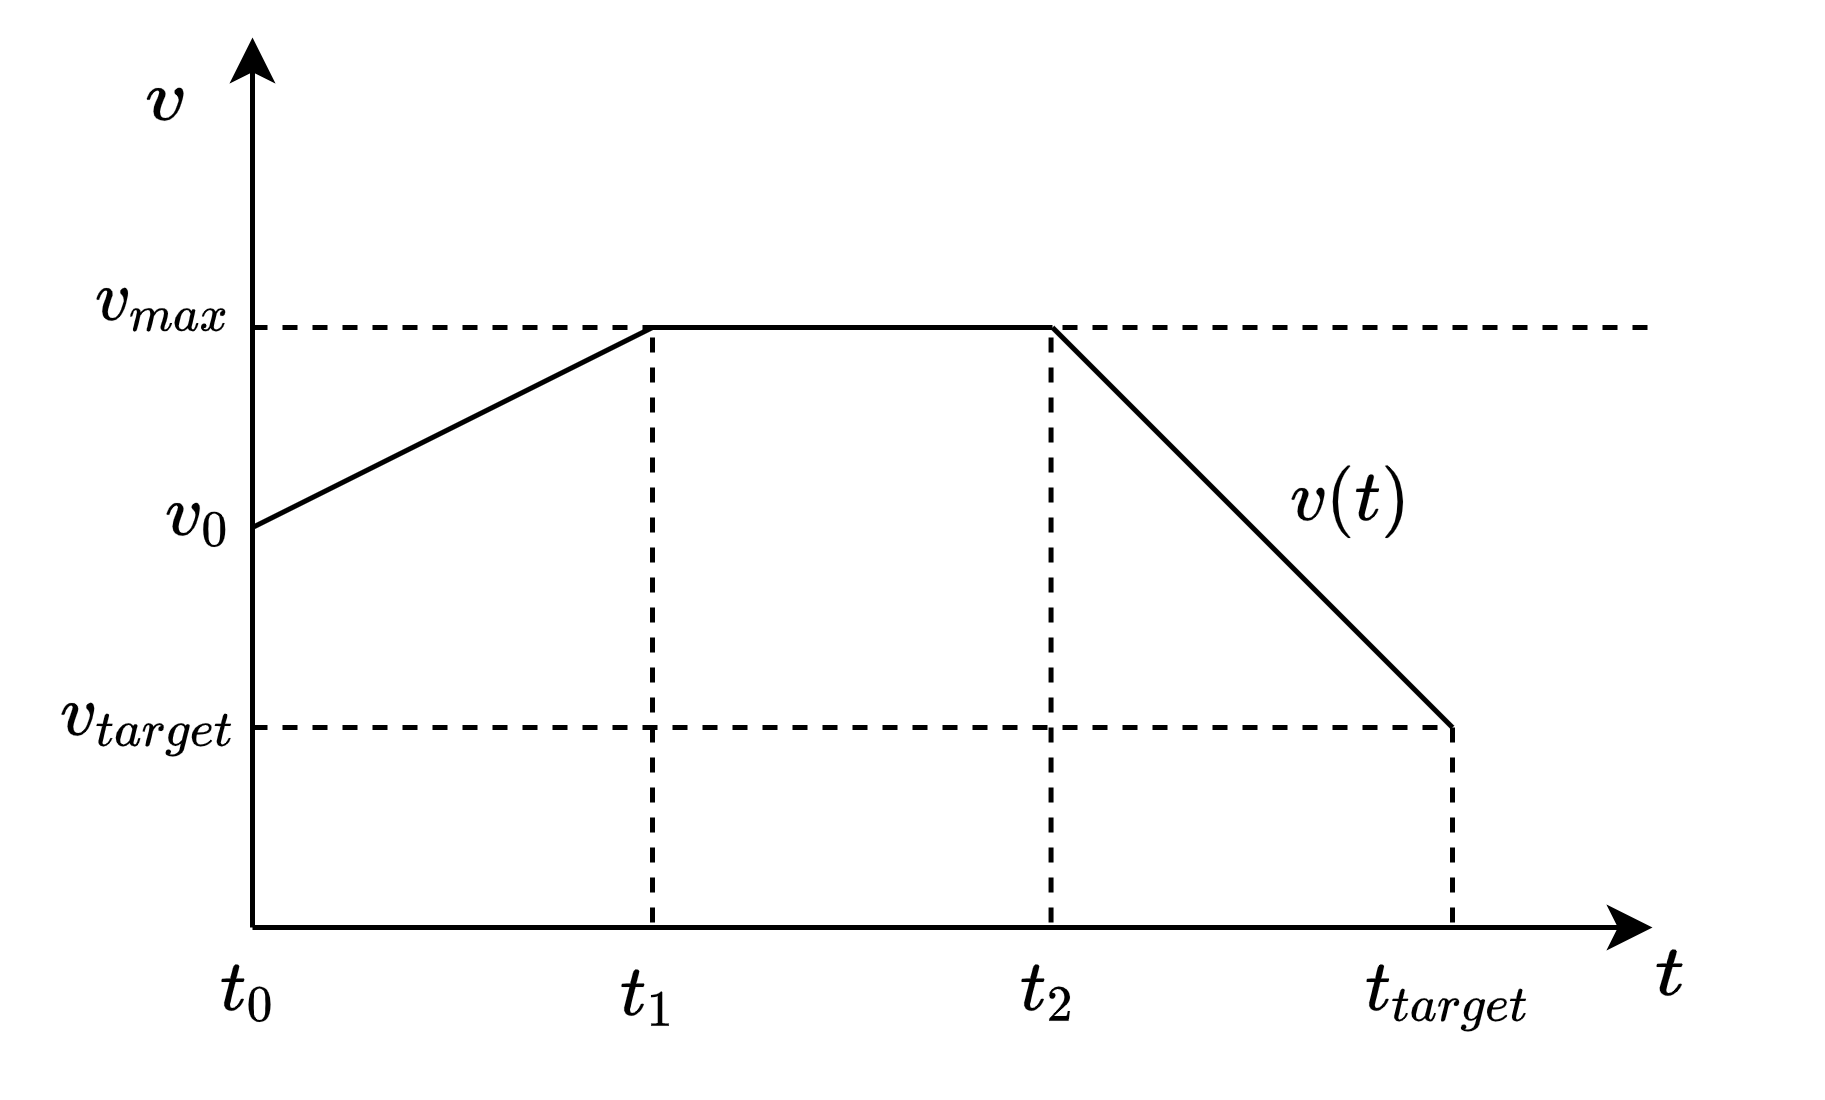
\includegraphics[width=0.7\textwidth]{figures/MotorSpeedCalculations/MSC_BCB_trajectory.png}
    \caption{Bang-coast-bang trajectory when $v_{max}$ is reached.}
    \label{fig: MSC_BCB}
\end{figure}

\noindent Now, filling in $v_0$ and $v_{target}$ in \cref{eq: tCrit,eq: sCrit} to obtain $t_{xy}$ and $s_{xy}$, the time/distance when moving from point $x$ to $y$:

\begin{align*}
    t_{01} &= t_{crit,0} = \frac{v_{max} - v_0}{a_{max}} \\
    t_{2target} &= t_{crit,target} = \frac{v_{max} - v_{target}}{a_{max}} \\
    s_{01} + s_{2target} &= s_{crit} = \frac{2 \, v_{max}^2+v_0^2 + v_{target}^2}{2 \, a_{max}}
\end{align*}

\noindent Then, the total duration from start of finish can be found, where the final result is shown in \cref{eq: tFastBCB}. 
\begin{align}
    s_{12} = s_{target} - s_{crit}  &= s_{target} - \frac{2 \, v_{max}^2-v_0^2 - v_{target}^2}{2 \, a_{max}} \nonumber \\
    t_{12} = \frac{s_{12}}{v_{max}} &= \frac{s_{target} - \frac{2 \, v_{max}^2-v_0^2 - v_{target}^2}{2 \, a_{max}}}{v_{max}} = \frac{s_{target}}{v_{max}} - \frac{v_{max}}{a_{max}} + \frac{v_0^2 + v_{target}^2}{2\, v_{max} \, a_{max}} \nonumber \\
    t_{0target} = t_{01} + t_{12} + t_{2target} &= \frac{v_{max} - v_0}{a_{max}}+ \frac{s_{target}}{v_{max}} - \frac{v_{max}}{a_{max}} + \frac{v_0^2 + v_{target}^2}{2\, v_{max} \, a_{max}} + \frac{v_{max} - v_{target}}{a_{max}}\nonumber \\
    &= \frac{v_{max} - v_0 - v_{target}}{a_{max}}+ \frac{s_{target}}{v_{max}} + \frac{v_0^2 + v_{target}^2}{2\, v_{max} \, a_{max}} \label{eq: tFastBCB}
\end{align}

\newpage
\subsection{Situation 2: Maximum Speed Not Reached} \label{sub: MSC_speednotreached}
\noindent In this situation, the motor does not reach $v_{max}$ and thus follows a bang-bang trajectory. The velocity of the motor over time in this situation is shown in \cref{fig: MSC_BCB}.
\begin{figure}[H]
    \centering
    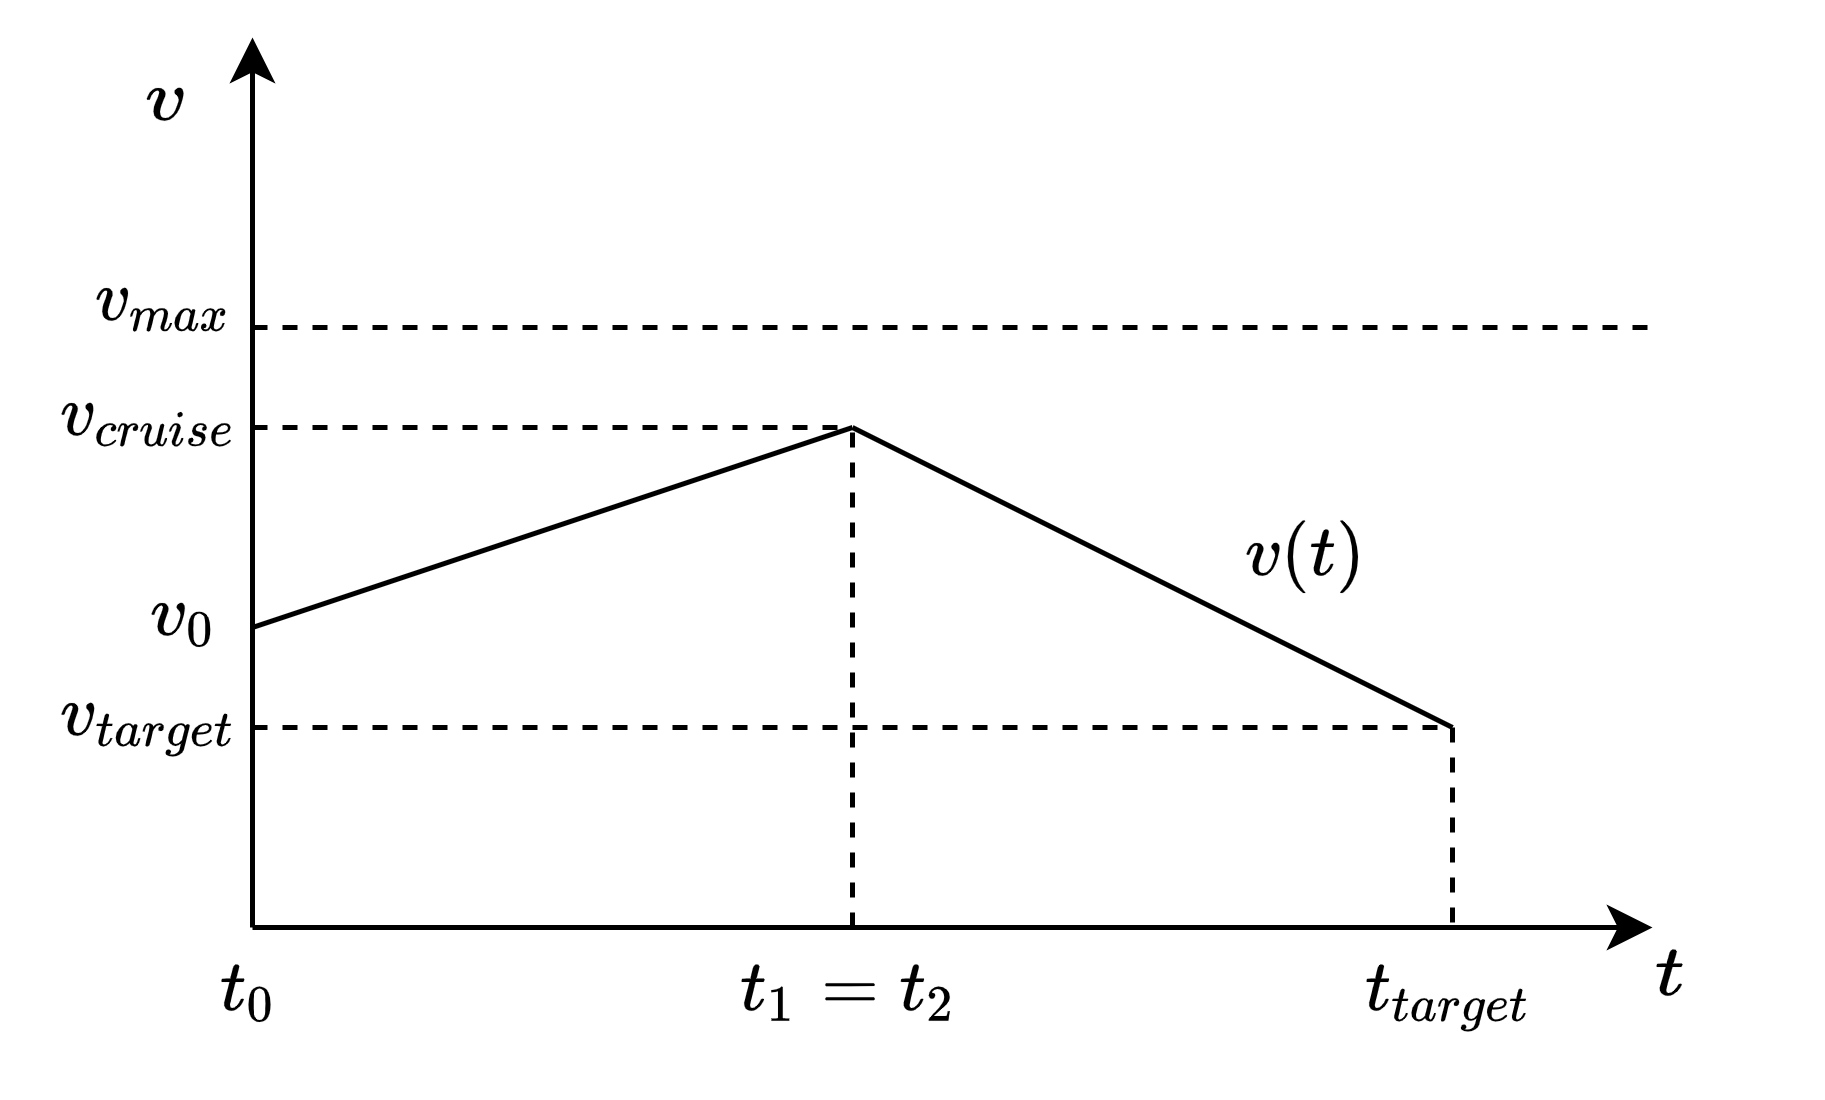
\includegraphics[width=0.7\textwidth]{figures/MotorSpeedCalculations/MSC_BB_trajectory.png}
    \caption{Bang-bang trajectory when $v_{max}$ is not reached.}
    \label{fig: MSC_BB}
\end{figure}

\noindent Because $v_{max}$ is not reached, its maximum reached speed is (currently) unknown. This speed, $v_{cruise}$, has to be chosen such that the desired distance is exactly traversed with the bang-bang trajectory. This can be done by expressing the distance as a function of $v_{cruise}$, which can be done by replacing all terms of $v_{max}$ in \cref{eq: tCrit,eq: sCrit} with $v_{cruise}$. The end result is shown in \cref{eq: tFastBB}. 
\begin{align}
    t_{01}  &= \frac{v_{cruise} - v_0}{a_{max}} \quad (\text{N.B.: }t_{12} = 0) \nonumber \\
    t_{2target}  &= \frac{v_{cruise} - v_{target}}{a_{max}} \nonumber \\
    s_{01} + s_{2target} = s_{target} &= \frac{2 \, v_{cruise}^2-v_0^2 - v_{target}^2}{2 \, a_{max}} \Rightarrow v_{cruise} = \sqrt{s_{target} \, a_{max} + \frac{1}{2}(v_0^2 + v_{target}^2)} \nonumber \\
t_{0target} = t_{01} + t_{2target} &= \frac{v_{cruise}-v_0}{a_{max}} + \frac{v_{cruise}-v_{target}}{a_{max}} = \frac{2 \, v_{cruise}-v_0 - v_{target}}{a_{max}}\nonumber \\
    &= \frac{2\,\sqrt{s_{target} \, a_{max} + \frac{1}{2}(v_0^2 + v_{target}^2)} -v_0 - v_{target} }{a_{max}} \label{eq: tFastBB}
\end{align}